\RequirePackage{amsmath}
\documentclass[runningheads]{llncs}

\usepackage{amssymb}
\usepackage{subfigure}
\usepackage{mathtools}
\usepackage{verbatim}
\usepackage{stmaryrd}
\usepackage{listings}
\usepackage{color}
\usepackage{courier}
\usepackage{xspace}

%\usepackage{amsmath, amssymb, amsfonts}
\usepackage{tikz}
\usetikzlibrary{automata}
\usepackage{filecontents}
\usepackage{listings}
\usepackage{stmaryrd}
\usepackage[margin=1in]{geometry}
%\usepackage{amsthm}

\definecolor{codegreen}{rgb}{0,0.6,0}
\definecolor{codegray}{rgb}{0.5,0.5,0.5}
\definecolor{codepurple}{rgb}{0.58,0,0.82}
\definecolor{backcolour}{rgb}{0.95,0.95,0.92}
\lstdefinestyle{mystyle}{
	stringstyle=\color{codepurple},
	basicstyle=\footnotesize\ttfamily,
	breakatwhitespace=false,         
	breaklines=true,                 
	captionpos=b,                    
	keepspaces=true,                
	numbersep=5pt,                  
	showspaces=false,                
	showstringspaces=false,
	showtabs=false,                  
	tabsize=2
}
\lstset{style=mystyle}

\newcommand\xqed[1]{\leavevmode\unskip\penalty9999 \hbox{}\nobreak\hfill\quad\hbox{#1}}
\newcommand\EOE{\xqed{$\clubsuit$}}
\newcommand\EOP{\xqed{$\square$}}

\newcommand{\dom}{\operatorname{dom}}
\newcommand{\im}{\operatorname{im}}
\newcommand{\sem}[1]{\ensuremath{\llbracket #1 \rrbracket}}
\renewcommand{\L}{{\cal L}}
\newcommand{\tc}{T_{\rm c\lca}}
\newcommand{\no}{{\tt null}}
\newcommand{\m}{\underline{m}}
\newcommand{\n}{\underline{n}}
\newcommand{\free}{\operatorname{free}}
\newcommand{\NN}{\mathbb{N}}
\newcommand{\C}{{\cal C}}
\newcommand{\D}{{\cal D}}
\newcommand{\B}{\mathbb{B}}
\newcommand{\F}{\mathbb{F}}
\newcommand{\K}{\mathbb{K}}
\newcommand{\V}{\mathbb{V}}
\newcommand{\W}{\mathbb{W}}

\newcommand{\defn}[1]{Definition~\ref{defn:#1}}
\newcommand{\fig}[2][]{Figure~\ref{fig:#2}\ensuremath{#1}}
\newcommand{\tab}[1]{Table~\ref{tab:#1}}
\newcommand{\eq}[1]{(\ref{eqn:#1})}
\newcommand{\ex}[1]{Example~\ref{ex:#1}}
\newcommand{\secn}[1]{Section~\ref{sec:#1}}
\newcommand{\lem}[1]{Lemma~\ref{lem:#1}}
\newcommand{\cor}[1]{Corollary~\ref{cor:#1}}
\newcommand{\thm}[1]{Theorem~\ref{thm:#1}}
\newcommand{\prop}[1]{Proposition~\ref{prop:#1}}

\newcommand{\ie}{i.e.,\xspace}
\newcommand{\eg}{\emph{e.g.}, \xspace}

%% I changed the symbols to 0,1,+,* to avoid confusion with the meet and join from lattices.
\newcommand{\cbot}{0}
\newcommand{\ctop}{1}
\newcommand{\ctimes}{\times}
\newcommand{\cplus}{+}
\newcommand{\CS}{{\bf CS}}

\pagestyle{plain}

%\long\def\/*#1*/{}

\lstdefinestyle{base}{
	emptylines=1,
	breaklines=false,
	basicstyle=\ttfamily\color{black},
	basicstyle=\footnotesize\ttfamily,
	moredelim=**[is][\color{red}]{@}{@},
}
\begin{document}

In this document, I give some examples of first-order definitions and how do they compose. I took the previous examples of Tobias, and ignored for now semiring values. Thus, soft constraints are considered as constraints. 


\paragraph{From automata to rules} \hspace{0pt} \\

\begin{figure}[!h]
\centering
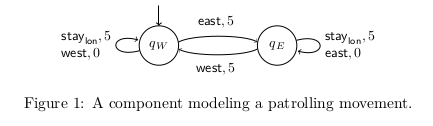
\includegraphics[scale=0.7]{Patrolling_movement.png}
\end{figure}
\noindent
According to the Component Action System, all actions of the soft constraint can be represented by a predicate over a set of ports.
Define a variable $s$ that indicates the current state. In $A_1$ automaton in Figure 1, $s_1=1$ refers to state $q_W$ and $s_1=2$ to state $q_E$.

Now, the automaton can be viewed as a single first-order formula :
\begin{align*}
\phi(A_1) =  & \quad ( s_1=1 \land ((east\land s_1'=2) \lor (west\ \land s_1'=1) \lor (stay_{lon}\land s_1'=1)) \lor  \\
	&\quad(s_1=2 \land ((east \land s_1'=2) \lor (west \land s_1'= 1 )\lor (stay_{lon} \land s_1'=2))) \\
	  =  & \quad r_1 \lor r_2 \lor r_3 \lor r_4 \lor r_5 \lor r_6,
\end{align*}

\noindent
with\\ 
$r_1 := s_1=1 \land (east\land s_1'=2)$ \\ \quad
$r_2 := s_1=1 \land (west\ \land s_1'=1)$ \\ \quad
$r_3 := s_1=1 \land (stay_{lon}\land s_1'=1)$\\ \quad
$r_4 := s_1=2 \land (east \land s_1'=2)$ \\ \quad
$r_5 := s_1=2 \land (west \land s_1'= 1 )$\\ \quad
$r_6 := s_1=2 \land (stay_{lon} \land s_1'=2)$\\ \quad
\begin{figure}[!h]
\centering
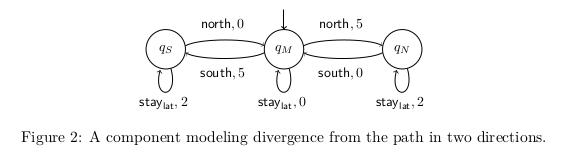
\includegraphics[scale=0.7]{divergence.png}
\end{figure}

\noindent
Similar to $A_1$ in Figure 1, automaton $A_2$ in Figure 2 can also be turned into a first-order formula. In automaton $A_2$, $s_2=1$ refers to state $q_M$, $s_2=2$ refers to state $q_S$ and $s_2=3$ refers to the state $q_N$.

\noindent
The corresponding formula is
\begin{align*}
\phi(A_2) =  & \quad ( s_2=1 \land ((south \land s_2'=2) \lor (stay_{lat}\land s_2'=1) \lor (north \land s_2'=3))  \\
	&\quad( s_2=2 \land ((north \land s_2'=1) \lor (stay_{lat}\land s_2'=2)) \\
	&\quad( s_2=3 \land ((south \land s_2'=1) \lor (stay_{lat}\land s_2'=3)) \\
	=  &\quad p_1 \lor p_2 \lor p_3 \lor p_4 \lor p_5 \lor p_6 \lor p_7 ,
\end{align*}

\noindent
with\\
$p_1 := s_2=1 \land (south \land s_2'=2)$\\ \quad
$p_2 := s_2=1 \land (north \land s_2'=3)$\\ \quad
$p_3 := s_2=1 \land (stay_{lat}\land s_2'=1)$\\ \quad
$p_4 := s_2=2 \land (north \land s_2'=1) $\\ \quad
$p_5 := s_2=2 \land (stay_{lat}\land s_2'=2)$\\ \quad
$p_6 := s_2=3 \land (south \land s_2'=1) $\\ \quad
$p_7 := s_2=3 \land (stay_{lat}\land s_2'=3) $\\ \quad


\paragraph{Composition of automata} \hspace{0pt} \\

The composition of $A_1$ and $A_2$ gives a new Component Automaton with 6 states (cartesian product of states from $A_1$ and $A_2$) and 42 transitions. From the logical perspective, composition only applies a composition operator on the formula of $A_1$ and the formula of $A_2$. 
For join composition, the operator is normal conjunction. The intuition behind this conjunction is that the new automaton must, for each transition, take a transition of $A_1$ and $A_2$. Then, assuming that automata are in disjunctive normal form and each clause represents a transition, a transition of $A$ is a transition of $A_1$ (one of its clauses) and a transition of $A_2$ (i.e. the conjunction of the two clauses). \\

For join composition, with $R = \{r_1, ..., r_6\}$ and $P=\{p_1, ...,p_7\}$  :
\begin{align*}
\phi(A)= &\quad \phi(A_1) \land \phi(A_2)\\
	\equiv & \quad (r_1 \lor r_2 \lor r_3 \lor r_4 \lor r_5 \lor r_6 ) \land (p_1 \lor p_2 \lor p_3 \lor p_4 \lor p_5 \lor p_6 \lor p_7)\\
	= & \quad \bigvee_{r_{i} \in R}r_i \land \bigvee_{p_i \in P} p_i\\
	= & \quad \bigvee_{r_{i} \in R, p_i \in P}r_i \land p_i
\end{align*}

More generally, for Soft Constraint Automata, the composition operator can be seen as a polymorphic operator $\otimes$, that behaves like a conjunction, except for soft constraints.
\begin{align*}
\phi(A)= &\quad \phi(A_1) \otimes \phi(A_2)\\
	= & \quad \bigvee_{r_{i} \in R}r_i \otimes \bigvee_{p_i \in P} p_i\\
	= & \quad \bigvee_{r_{i} \in R, p_i \in P}r_i \otimes p_i
\end{align*}

We assume that $\otimes$ distributes over $\land$, hence the first product $r_1 \otimes p_1$ is :
\begin{align*}
 r_1 \otimes p_1 =&\quad (s_1=1 \land (east\land s_1'=2)) \otimes (s_2=1 \land (south \land s_2'=2))\\
		 =&\quad s_1=1 \otimes s_2=1 \land (east\land s_1'=2) \otimes (south \land s_2'=2)\\
		 =&\quad s_1=1 \land s_1'=2 \land s_2=1 \land s_2'=2 \land east \otimes south 
\end{align*}

The polymorphic operator $\otimes$ should evalute to a different operator regarding the type of the actions. In this example, if the type of action $east$ is Longitude and the type of action $south$ is Latitude, by defining a type hierarchy, $\otimes$ has different interpretations. If Longitude is prefered as Latitude, $\otimes$ would be evaluated to $\rhd$. If the types are equals, then $\otimes$ is evaluated to $\land$.

Composition must also take care of semiring value composition. At this point, I don't see yet how to properly integrate soft constraint inside those formula.
\end{document}


